\documentclass{article}
\def\pgfsysdriver{pgfsys-tex4ht.def}
\usepackage{tikz,amsmath, amssymb,bm,color}
\usepackage[margin=0cm,nohead]{geometry}
% \usepackage[active,tightpage]{preview}
\usetikzlibrary{shapes,arrows}
% needed for BB
\usetikzlibrary{calc}

% \PreviewEnvironment{tikzpicture}

\begin{document}
\usetikzlibrary{arrows}
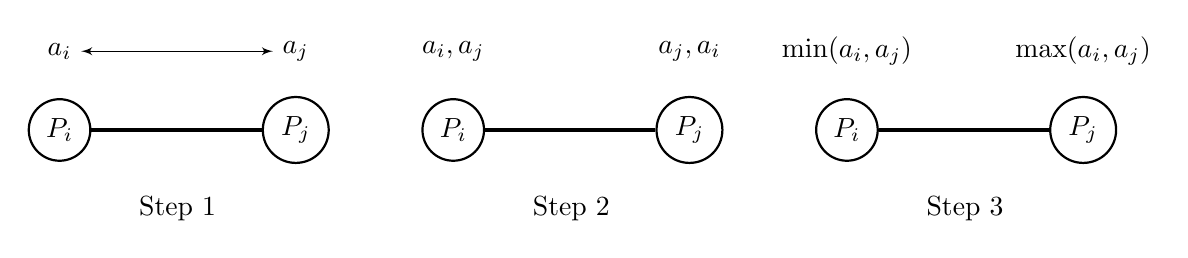
\begin{tikzpicture}

\node (v1) at (-5,0) {$a_i$};
\node (v2) at (-2,0) {$a_j$};

\node[draw, thick, circle] (P1) at (-5,-1) {$P_i$};
\node[draw, thick, circle] (P2) at (-2,-1) {$P_j$};

\draw [latex'-latex', double] (v1) edge (v2);


\draw[ultra thick]  (P1) edge (P2);

\node at (-3.5,-2) {Step 1};

\begin{scope}[shift={(5,0)}]

\node (v1) at (-5,0) {$a_i,a_j$};
\node (v2) at (-2,0) {$a_j,a_i$};

\node[draw, thick, circle] (P1) at (-5,-1) {$P_i$};
\node[draw, thick, circle] (P2) at (-2,-1) {$P_j$};

\draw[ultra thick]  (P1) edge (P2);

\node at (-3.5,-2) {Step 2};
\end{scope}

\begin{scope}[shift={(10,0)}]

\node (v1) at (-5,0) {$\min(a_i, a_j)$};
\node (v2) at (-2,0) {$\max(a_i, a_j)$};

\node[draw, thick, circle] (P1) at (-5,-1) {$P_i$};
\node[draw, thick, circle] (P2) at (-2,-1) {$P_j$};

\draw[ultra thick]  (P1) edge (P2);

\node at (-3.5,-2) {Step 3};
\end{scope}

\end{tikzpicture}
\end{document}
